%%%%%%%%%%%%%%%%%%%%%%%%%%%%%%%%%%%%%%%%%%
% Mathematics Final Year Research Projects
% LaTeX Template
% Version 1.0 (31/01/24)
%
% This template has been adapted from: https://www.overleaf.com/latex/templates/imperial-college-report-template/wncnzptkhnbc
% Students should feel free to adapt this template to their needs.
%%%%%%%%%%%%%%%%%%%%%%%%%%%%%%%%%%%%%%%%%%
%----------------------------------------------------------------------------------------
% PACKAGES AND OTHER DOCUMENT CONFIGURATIONS
%----------------------------------------------------------------------------------------
\documentclass[a4paper,11pt, twoside]{report}

%% Language and font encodings
\usepackage[english]{babel}
\usepackage[utf8]{inputenc}
\usepackage[T1]{fontenc}

%% Imperial Recommended Packages
\usepackage{afterpage}

% Lean colour configurations
\usepackage{color}
\definecolor{keywordcolor}{rgb}{0.7, 0.1, 0.1}   % red
\definecolor{tacticcolor}{rgb}{0.0, 0.1, 0.6}    % blue
\definecolor{commentcolor}{rgb}{0.4, 0.4, 0.4}   % grey
\definecolor{symbolcolor}{rgb}{0.0, 0.1, 0.6}    % blue
\definecolor{sortcolor}{rgb}{0.1, 0.5, 0.1}      % green
\definecolor{attributecolor}{rgb}{0.7, 0.1, 0.1} % red
\definecolor{backcolour}{rgb}{0.95,0.95,0.92}

% Listings (for displaying code):
\usepackage{listings}
\def\lstlanguagefiles{TeX_Setup/lstlean.tex}
\lstset{
    % frame = single, 
    % framexleftmargin=15pt,
    language = lean,
    numbers = left,
    backgroundcolor=\color{backcolour}
}

% ----------- Algorithm2e setup
\usepackage[ruled,vlined]{algorithm2e}
\makeatletter
\renewcommand{\SetKwInOut}[2]{%
  \sbox\algocf@inoutbox{\KwSty{#2}\algocf@typo:}%
  \expandafter\ifx\csname InOutSizeDefined\endcsname\relax% if first time used
    \newcommand\InOutSizeDefined{}\setlength{\inoutsize}{\wd\algocf@inoutbox}%
    \sbox\algocf@inoutbox{\parbox[t]{\inoutsize}{\KwSty{#2}\algocf@typo:\hfill}~}\setlength{\inoutindent}{\wd\algocf@inoutbox}%
  \else% else keep the larger dimension
    \ifdim\wd\algocf@inoutbox>\inoutsize%
    \setlength{\inoutsize}{\wd\algocf@inoutbox}%
    \sbox\algocf@inoutbox{\parbox[t]{\inoutsize}{\KwSty{#2}\algocf@typo:\hfill}~}\setlength{\inoutindent}{\wd\algocf@inoutbox}%
    \fi%
  \fi% the dimension of the box is now defined.
  \algocf@newcommand{#1}[1]{%
    \ifthenelse{\boolean{algocf@inoutnumbered}}{\relax}{\everypar={\relax}}%
%     {\let\\\algocf@newinout\hangindent=\wd\algocf@inoutbox\hangafter=1\parbox[t]{\inoutsize}{\KwSty{#2}\algocf@typo\hfill:}~##1\par}%
    {\let\\\algocf@newinout\hangindent=\inoutindent\hangafter=1\parbox[t]{\inoutsize}{\KwSty{#2}\algocf@typo:\hfill}~##1\par}%
    \algocf@linesnumbered% reset the numbering of the lines
  }}%
\makeatother
% --------- end algorithm2e setup

\usepackage{bm}
\usepackage[normalem]{ulem}

\usepackage[colorinlistoftodos]{todonotes}

% I have all of their other recommended packages somewhere on here.

\usepackage[most]{tcolorbox}
\usepackage{authblk}  % Lets you add an \affil{} to your title, stating your affiliation {eg. Sigma Mathematics Society}
\usepackage{ragged2e}
\usepackage{csquotes}
\usepackage{pdfpages}



\usepackage{xfrac}
\usepackage{cancel}

\usepackage[inline]{enumitem}

%\usepackage{tgpagella}

\usepackage{blindtext}
\usepackage{lipsum}
\usepackage{verbatim}
\usepackage{hyperref}
\hypersetup{
    citebordercolor = 1 1 1,
    linkbordercolor = 1 1 1,
    filebordercolor = 1 1 1,
    menubordercolor = 1 1 1,
    urlbordercolor = 1 1 1,
    colorlinks  =   true,
    linkcolor   =   blue,
    citecolor   =   magenta,
    urlcolor    =   blue
}

% This project uses natbib instead. See end of format file.
% \usepackage{biblatex} % Modify citation format using [style=yourstyle] parameter--eg \usepackage[style=mla-new]{biblatex}
% \bibliography{TeX_Setup/References.bib}
% \addbibresource{TeX_Setup/References.bib}

\usepackage{cancel}
\usepackage{amssymb}
\usepackage{amsmath}
% \usepackage{amsthm}  % In `environments.tex`
%\usepackage{MnSymbol}
\usepackage{mathrsfs}
\usepackage{mathtools}
% \usepackage{mathabx}
\usepackage{mathdots}
\usepackage{yhmath}

\usepackage{array}
\usepackage{booktabs}
\usepackage{longtable}

\usepackage{graphicx}
\newcommand\sbullet[1][.5]{\mathbin{\vcenter{\hbox{\scalebox{#1}{$\bullet$}}}}}  % Bullet of customisable size
\usepackage{wrapfig}
% Imperial-recommended `caption` setup
\usepackage{caption}
\captionsetup[figure]{labelfont={bf}, name={Figure}, justification=centering}
\captionsetup[table]{labelfont={bf}, name={Table}}
\usepackage{subcaption}
\usepackage{tikz}
\usepackage{float}

% Tikz
\usepackage{tikz-cd}
\usepackage{tikz-3dplot}
\usetikzlibrary{positioning}
\usetikzlibrary{cd}
\usetikzlibrary{shapes.geometric}
\usepackage{pgfplots}
\usepackage{mathrsfs}
\usetikzlibrary{arrows}
\usepackage{qtree}

%% Sets page size and margins
\usepackage[a4paper,top=1in,bottom=1in,left=1in,right=1in,marginparwidth=1.75cm]{geometry}

% Font

% \usepackage{sansmathfonts}
% % \usepackage{mathrsfs}
% \usepackage[T1]{fontenc}
% \renewcommand*\familydefault{\sfdefault}

\renewcommand*{\rmdefault}{bch}
\renewcommand*{\ttdefault}{lmtt}

% Structure and Numbering

\usepackage{fancyhdr}
\usepackage{lastpage}

\pagestyle{fancy}
\fancyhf{}

\rhead{{Page \thepage}}%\hspace{1pt} of \pageref{LastPage}}}
\lhead{\textit\slshape\nouppercase{\leftmark}}

\numberwithin{equation}{section}

% Lists

\setlist[description]{font=\normalfont}
\setlist[enumerate]{before=\normalfont}

% Spacing and indentation

% Not sure if 1.5-spacing is permitted. I'll leave it commented out for now.
% \usepackage{setspace}
% \renewcommand{\baselinestretch}{1.5}

\usepackage[skip=11pt, indent=0pt]{parskip}
% Here's what Imperial's recommended setup is:
% \setlength{\parskip}{0.5em}
% \usepackage{indentfirst}  % Uncomment if using above

\allowdisplaybreaks  % Allows align environments to continue for several pages

% Colours

\usepackage{xcolor}
\definecolor{darkblue}{rgb}{0.0, 0.0, 0.55}
\definecolor{pink}{rgb}{0.858, 0.188, 0.478}
\definecolor{brown}{rgb}{0.8, 0.4, 0.0}

% Bibliography
\usepackage[numbers, comma, square, sort&compress]{natbib}
\bibliographystyle{References/abbrvunsrtnat.bst}
% \bibliographystyle{unsrtnat}

\usepackage{amsthm}
% Gives theorem and definition names the same font style as the words "theorem"/"definition": see https://tex.stackexchange.com/questions/43966/how-to-make-the-optional-title-of-a-theorem-bold-with-amsthm
\makeatletter
\def\th@plain{%
  \thm@notefont{}% same as heading font
  \itshape % body font
}
\def\th@definition{%
  \thm@notefont{}% same as heading font
  \normalfont % body font
}
\makeatother

\usepackage{cleveref}

\newtheorem*{theorem*}{Theorem}
\newtheorem{theorem}{Theorem}[section]
\newtheorem{corollary}[theorem]{Corollary}%[theorem]
\newtheorem{lemma}[theorem]{Lemma}
\newtheorem{claim}[theorem]{Claim}
\newtheorem{conjecture}[theorem]{Conjecture}
% \newtheorem{algorithm}[theorem]{Algorithm}  % Defined in algorithm2e
\newtheorem{proposition}[theorem]{Proposition}

\newtheorem{problem}[theorem]{Problem}
\newenvironment{boxproblem}{
    \begin{tcolorbox}[colback=yellow!15!white,colframe=orange, breakable, enhanced]\begin{problem}
}{
    \end{problem}\end{tcolorbox}
}

\newenvironment{boxtheorem}{
    \begin{tcolorbox}[colback=yellow!15!white,colframe=orange, breakable, enhanced]\begin{theorem}
}{
    \end{theorem}\end{tcolorbox}
}
\newenvironment{boxproposition}{
    \begin{tcolorbox}[colback=yellow!15!white,colframe=orange, breakable, enhanced]\begin{proposition}
}{
    \end{proposition}\end{tcolorbox}
}
\newenvironment{boxlemma}{
    \begin{tcolorbox}[colback=yellow!15!white,colframe=orange, breakable, enhanced]\begin{lemma}
}{
    \end{lemma}\end{tcolorbox}
}
\newenvironment{boxcorollary}{
    \begin{tcolorbox}[colback=yellow!15!white,colframe=orange, breakable, enhanced]\begin{corollary}
}{
    \end{corollary}\end{tcolorbox}
}
\newenvironment{boxconjecture}{
    \begin{tcolorbox}[colback=yellow!15!white,colframe=orange, breakable, enhanced]\begin{conjecture}
}{
    \end{conjecture}\end{tcolorbox}
}


\theoremstyle{remark}
\newtheorem*{remark}{Remark}
\newtheorem*{solution}{Solution}

\theoremstyle{definition}
\newtheorem{definition}[theorem]{Definition}
\newenvironment{boxdefinition}{
    \begin{tcolorbox}[colback=cyan!10!white,colframe=cyan!70!black, breakable, enhanced]\begin{definition}
}{
    \end{definition}\end{tcolorbox}
}
\newtheorem*{convention}{Convention}
\newenvironment{boxconvention}{
    \begin{tcolorbox}[colback=magenta!3!white,colframe=magenta!70!black, breakable, enhanced]\begin{convention}
}{
    \end{convention}\end{tcolorbox}
}
\newtheorem*{notation}{Notation}
\newenvironment{boxnotation}{
    \begin{tcolorbox}[colback=magenta!3!white,colframe=magenta!70!black, breakable, enhanced]\begin{notation}
}{
    \end{notation}\end{tcolorbox}
}
\newtheorem{example}[theorem]{Example}
\newenvironment{boxexample}{
    \begin{tcolorbox}[colframe=green!30!black, breakable, enhanced, breakable, enhanced]\begin{example}
}{
    \end{example}\end{tcolorbox}
}
\newtheorem{nexample}[theorem]{Non-Example}
\newenvironment{boxnexample}{
    \begin{tcolorbox}[colframe=red!50!black, breakable, enhanced]\begin{nexample}
}{
    \end{nexample}\end{tcolorbox}
}
\newtheorem{cexample}[theorem]{Counterexample}
\newenvironment{boxcexample}{
    \begin{tcolorbox}[colframe=red!50!black, breakable, enhanced]\begin{cexample}
}{
    \end{cexample}\end{tcolorbox}
}

% \def\SMALLCOLWIDTH{1.5cm}
\newcolumntype{C}[1]{>{\centering\let\newline\\\arraybackslash\hspace{0pt}}m{#1}}

% Centering captions
% \renewcommand{\caption}[1]{\caption{\centering #1}}

%%%%%%%%%%%%%%%%%%%%%%%%%%%%%%%%%%%%%%%%%%%%%%%%%%%%%%%%%%%%%%%%%%%%%%%%%%%%%%%%%%%%%%%%%%%%%%%%%%%%%%%%%%%%
% CUSTOM COMMANDS
%%%%%%%%%%%%%%%%%%%%%%%%%%%%%%%%%%%%%%%%%%%%%%%%%%%%%%%%%%%%%%%%%%%%%%%%%%%%%%%%%%%%%%%%%%%%%%%%%%%%%%%%%%%%

% Custom colours

\definecolor{darkgreen}{rgb}{0.1, 0.4, 0.3}      % green

% `sorry`

\newcommand{\sorry}{\textcolor{red}{\texttt{sorry}}}
% \newcommand{\sorry}{\lstinline{sorry}}

% TIKZ:

\newcommand{\drawplane}{  % For use with TikZ
    \draw[step=0.5cm,gray,very thin] (-2.5,-2.5) grid (2.5,2.5);
    \draw[thick,->] (-2.5,0) -- (2.5,0); % node[anchor=west] {$x$};
    \draw[thick,->] (0,-2.5) -- (0,2.5); % node[anchor=south] {$y$};
    % \node[black, anchor=north east] at (0, 0) {$0$};
}
\newcommand{\latticecircle}[2]{
    \draw[fill=yellow, opacity=0.5] (#1, #2) circle (0.5);
    \node at (#1, #2) {\color{gray}{$\bullet$}};
}
\newcommand{\latticecirclegrey}[2]{
    \draw[fill=gray, opacity=0.75] (#1, #2) circle (0.5);
    \node at (#1, #2) {\color{black}{$\bullet$}};
}
\newcommand{\latticecirclebrown}[2]{
    \draw[fill=brown, opacity=0.75] (#1, #2) circle (0.5);
    \node at (#1, #2) {\color{black}{$\bullet$}};
}
\usetikzlibrary{decorations.markings}
\tikzset{->-/.style={decoration={
      markings,
      mark=at position #1 with {\arrow{>}}},postaction={decorate}
}}

\newenvironment{cd}{
    \begin{equation} \begin{tikzcd}
}{
    \end{tikzcd} \end{equation}
}
\newenvironment{cd*}{
    \begin{equation*} \begin{tikzcd}
}{
    \end{tikzcd} \end{equation*}
}

\newcommand{\drawsquare}[1]{
    \draw[thick, blue]
    (-{#1},-{#1}) node [anchor=north east] {C} --
    (-{#1}, {#1}) node[anchor=south east] {B} --
    ({#1}, {#1}) node[anchor=south west] {A} --
    ({#1}, -{#1}) node [anchor=north west] {D} -- cycle;
}

\newcommand{\labelledpoint}[5]{ % Takes x coord, y coord, label x-position relative to point, label y-position relative to point, label text as arguments
    \node [label={[shift={(#3,#4)}]#5}] at (#1, #2) {$\bullet$};
}

% DELIMITERS:

\newcommand{\parenth}[1]{\left( #1 \right)}
\newcommand{\brac}[1]{\left[ #1 \right]}
\newcommand{\set}[1]{\left\{ #1 \right\}}
\newcommand{\setst}[2]{\set{#1 \; \middle\vert \; #2}}
\newcommand{\abs}[1]{\left\lvert #1 \right\rvert}
\newcommand{\norm}[1]{\left\lVert #1 \right\rVert}
\newcommand{\floor}[1]{\left\lfloor #1 \right\rfloor}
\newcommand{\ceil}[1]{\left\lceil #1 \right\rceil}
\newcommand{\cycl}[1]{\left\langle #1 \right\rangle}
\newcommand{\grpres}[2]{\cycl{#1 \; \middle| \; #2}}  % \grpres{gens}{rels}

% FUNCTIONS:

\newcommand{\fx}{f\!\parenth{x}}
\newcommand{\fof}[1]{f\!\parenth{#1}}

\newcommand{\px}{p\!\parenth{x}}
\newcommand{\pof}[1]{p\!\parenth{#1}}
\newcommand{\pofbig}[1]{p\Big(#1\Big)}
\newcommand{\gx}{g\!\parenth{x}}
\newcommand{\gof}[1]{g\!\parenth{#1}}
\newcommand{\hx}{h\!\parenth{x}}
\newcommand{\hof}[1]{h\!\parenth{#1}}
\newcommand{\Tv}{T\!\parenth{v}}
\newcommand{\Tof}[1]{T\!\parenth{#1}}
\newcommand{\Tbar}{\overline{T}}
\newcommand{\Tbarof}[1]{\Tbar\!\parenth{#1}}
\newcommand{\Tbarv}{\Tbarof{v}}
\newcommand{\Sof}[1]{S\!\parenth{#1}}

\newcommand{\psin}[1]{\sin\!{\parenth{#1}}}
\newcommand{\pcos}[1]{\cos\!{\parenth{#1}}}
\newcommand{\ptan}[1]{\tan\!{\parenth{#1}}}
\newcommand{\sinsq}[1]{\sin^2\!\parenth{#1}}
\newcommand{\cossq}[1]{\cos^2\!\parenth{#1}}
\newcommand{\tansq}[1]{\tan^2\!\parenth{#1}}
\newcommand{\parcsin}[1]{\arcsin\!{\parenth{#1}}}
\newcommand{\parccos}[1]{\arccos\!{\parenth{#1}}}
\newcommand{\parctan}[1]{\arctan\!{\parenth{#1}}}

\newcommand{\logbase}[2]{\log_{#1}\!\parenth{#2}}
\newcommand{\nthroot}[2]{\sqrt[\leftroot{-3}\uproot{3} #1]{#2}}
\newcommand{\cbrt}[1]{\nthroot{3}{#1}}

\newcommand{\pgcd}[2]{\gcd\!\parenth{{#1},{#2}}}
\newcommand{\plcm}[2]{\operatorname{lcm}\!\parenth{{#1},{#2}}}
\newcommand{\pgcds}[1]{\gcd\!\parenth{#1}}
\newcommand{\plcms}[1]{\operatorname{lcm}\!\parenth{#1}}

\newcommand{\varphiof}[1]{\varphi\!\parenth{#1}}
\newcommand{\phiof}[1]{\phi\!\parenth{#1}}
\newcommand{\xiof}[1]{\xi\!\parenth{#1}}
\newcommand{\rhoof}[1]{\rho\!\parenth{#1}}
\newcommand{\pexp}[1]{\exp\!\parenth{#1}}

\newcommand{\inj}{\hookrightarrow}
\newcommand{\surj}{\twoheadrightarrow}

\DeclareMathOperator*{\argmin}{\arg\!\min}
\DeclareMathOperator*{\argmax}{\arg\!\max}

\newcommand{\of}[1]{\!\parenth{#1}}

% CALCULUS:

\newcommand{\dx}{\operatorname{d}\!x}
\newcommand{\dy}{\operatorname{d}\!y}
\newcommand{\diff}[1]{\operatorname{d}\!{#1}}
\newcommand{\dydx}{\frac{\dy}{\dx}}

% LINEAR ALGEBRA:

\newcommand{\mat}[3]{\operatorname{M}_{{#1} \times {#2}}\!\parenth{{#3}}}
\newcommand{\matsq}[2]{\operatorname{M}_{{#1} \times {#1}}\!\parenth{\mathbb{#2}}}
\newcommand{\MnR}{\operatorname{M}_{n}\!\parenth{\real}}
\newcommand{\MnC}{\operatorname{M}_{n}\!\parenth{\C}}
\newcommand{\Mn}[2]{\operatorname{M}_{#1}\!\parenth{#2}}
\newcommand{\GL}[1]{\operatorname{GL}\!\parenth{#1}}
\newcommand{\SL}[1]{\operatorname{SL}\!\parenth{#1}}
\newcommand{\PGL}[1]{\operatorname{PGL}\!\parenth{#1}}
\newcommand{\PSL}[1]{\operatorname{PSL}\!\parenth{#1}}

\newcommand{\Span}[1]{\operatorname{Span}\!\parenth{#1}}

\newcommand{\pdim}[1]{\dim\!\parenth{#1}}

\newcommand{\RSp}[1]{\operatorname{RSp}\!\parenth{#1}}
\newcommand{\CSp}[1]{\operatorname{CSp}\!\parenth{#1}}
\newcommand{\rank}[1]{\operatorname{rank}\!\parenth{#1}}
\newcommand{\pim}[1]{\operatorname{im}\!\parenth{#1}}
\newcommand{\pker}[1]{\operatorname{ker}\!\parenth{#1}}
\newcommand{\pdet}[1]{\det\!\parenth{#1}}

\newcommand{\cA}[1]{c_A \! \parenth{#1}}
\newcommand{\cB}[1]{c_B \! \parenth{#1}}
\newcommand{\mA}[1]{m_A \! \parenth{#1}}
\newcommand{\mB}[1]{m_B \! \parenth{#1}}
\newcommand{\cAx}{\cA{x}}
\newcommand{\cBx}{\cB{x}}
\newcommand{\mAx}{\mA{x}}
\newcommand{\mBx}{\mB{x}}
\newcommand{\cof}[2]{c_{#1}\!\parenth{#2}}
\newcommand{\mof}[2]{m_{#1}\!\parenth{#2}}

\newcommand{\Cof}[1]{C\!\parenth{#1}}
\newcommand{\+}{\oplus}
\newcommand{\pdeg}[1]{\deg\!\parenth{#1}}

\newcommand{\RCF}[1]{\operatorname{RCF}\!\parenth{#1}}
\newcommand{\JCF}[1]{\operatorname{JCF}\!\parenth{#1}}

\newcommand{\Jsub}[2]{J_{#1}\!\parenth{#2}}

\newcommand{\Aof}[1]{A\!\parenth{#1}}

\newcommand{\Tsub}[2]{T_{#1}\!\parenth{#2}}

\newcommand{\Tr}[1]{\operatorname{Tr}\!\parenth{#1}}

\newcommand{\diag}[1]{\operatorname{diag}\!\parenth{#1}}

% Measure Theory

\newcommand{\muof}[1]{\mu\!\parenth{#1}}
\newcommand{\muA}{\muof{A}}
\newcommand{\muB}{\muof{B}}
\newcommand{\mutof}[1]{\Tilde{\mu}\!\parenth{#1}}
\newcommand{\mustof}[1]{\mu^*\!\parenth{#1}}
\newcommand{\calF}{\mathcal{F}}
\newcommand{\calA}{\mathcal{A}}
\newcommand{\calB}{\mathcal{B}}
\newcommand{\calC}{\mathcal{C}}
\newcommand{\sigmaof}[1]{\sigma\!\parenth{#1}}
\newcommand{\psiof}[1]{\psi\!\parenth{#1}}

% Intervals

\newcommand{\Ioc}[1]{\left(#1\right]}
\newcommand{\Ico}[1]{\left[#1\right)}

% GROUPS/ALGEBRA IN GENERAL:

\newcommand{\inv}{^{-1}}
\newcommand{\Sym}[1]{\operatorname{Sym}\!\parenth{#1}}
\newcommand{\ord}[1]{\operatorname{ord}\!\parenth{#1}}
\newcommand{\supp}[1]{\operatorname{supp}\!\parenth{#1}}
\newcommand{\sgn}[1]{\operatorname{sgn}\!\parenth{#1}}
\newcommand{\tcyc}[2]{\begin{pmatrix} #1 & #2 \end{pmatrix}}

\newcommand{\nsg}{\trianglelefteq}

\newcommand{\Rmul}{R^{\times}}
\newcommand{\kmul}{k^{\times}}
\newcommand{\kX}{k\!\brac{X}}
\newcommand{\RX}{R\!\brac{X}}

\newcommand{\quotient}[2]{
    \left.\raisebox{.2em}{${#1}$} \middle/ \raisebox{-.2em}{${#2}$} \right.
}
\newcommand{\Zmod}[1]{\quotient{\Z}{{#1}\Z}}

\newcommand{\Vof}[1]{V\!\parenth{#1}}

\newcommand{\Frac}[1]{\operatorname{Frac}\!\parenth{#1}}

\newcommand{\Spec}[1]{\operatorname{Spec}\!\parenth{#1}}

\newcommand{\id}{\operatorname{id}}

\newcommand{\pchar}[1]{\operatorname{char}\!\parenth{#1}}

\newcommand{\Hom}{\operatorname{Hom}}

\newcommand{\Zof}[1]{\operatorname{Z}\!\parenth{#1}}

\newcommand{\Aut}[1]{\operatorname{Aut}\!\parenth{#1}}

% NUMBER SETS:

\newcommand{\real}{\mathbb{R}}
\newcommand{\rational}{\mathbb{Q}}
\newcommand{\naturalnum}{\mathbb{N}}
\newcommand{\integers}{\mathbb{Z}}
\newcommand{\complex}{\mathbb{C}}

\newcommand{\Field}{\mathbb{F}}
\newcommand{\Q}{\mathbb{Q}}
\newcommand{\R}{\real}
\newcommand{\N}{\naturalnum}
\newcommand{\Z}{\integers}
\newcommand{\C}{\complex}
\newcommand{\B}{\mathcal{B}}
\newcommand{\I}{\mathcal{I}}
\newcommand{\J}{\mathcal{J}}

\newcommand{\psup}[1]{\sup\!\parenth{#1}}
\newcommand{\pinf}[1]{\inf\!\parenth{#1}}

% LOGIC:

\newcommand{\ergo}{\therefore}
\newcommand{\bcos}{\because}
\newcommand{\st}{\text{ s.t. }}


% -------------------- SPECIFIC TO PROJECT -------------------- %

% TERMINOLOGY

\newcommand{\CELP}{Cohn-Elkies Linear Programming Bound}
\newcommand{\CEC}{Cohn-Elkies Conditions}
\newcommand{\JCT}{Jordan Curve Theorem}
\newcommand{\CGT}{Cauchy-Goursat Theorem}

% NOTATION

\newcommand{\Pa}{\mathcal{P}}
\newcommand{\Vol}{\operatorname{Vol}}
\newcommand{\Volof}[1]{\Vol\!\parenth{#1}}
\newcommand{\Sch}{\mathcal{S}}
\renewcommand{\hat}{\widehat}
\renewcommand{\tilde}{\widetilde}
\newcommand{\F}{\mathcal{F}}
\newcommand{\periodic}{\operatorname{periodic}}

\newcommand{\Halfplane}{\mathbb{H}} % Using Lean notation for the upper-half plane instead of Viazovska's

\newcommand{\BigO}[1]{\operatorname{O}\of{#1}}

\newcommand{\fm}{f \mid}
\newcommand{\fmof}[3]{\parenth{\fm_{#1} {#2}}\of{#3}}

% COMPLEX ANALYSIS

\renewcommand{\Re}{\operatorname{Re}}
\renewcommand{\Im}{\operatorname{Im}}

\newcommand{\rad}{_{\operatorname{rad}}}

% LEAN

\newcommand{\mathlib}{\texttt{mathlib}}


% %% Useful packages
% \usepackage{afterpage}
% \usepackage{amsmath}
% \usepackage{amsthm}
% \usepackage{amssymb}
% \usepackage{csquotes}
% \usepackage{enumitem}
% \usepackage{graphicx}
% \usepackage{lipsum}
% \usepackage{booktabs}

% % Listings (for displaying code):
% \usepackage{listings}
% \lstset{
%     frame = single, 
%     framexleftmargin=15pt
% }

% % Center figure captions:
% \usepackage{caption}
% \captionsetup[figure]{labelfont={bf},name={Figure},labelsep=quad}
% \captionsetup[table]{labelfont={bf},name={Table},labelsep=quad}


% % ----------- Algorithm2e setup
% \usepackage[ruled,vlined]{algorithm2e}
% \makeatletter
% \renewcommand{\SetKwInOut}[2]{%
%   \sbox\algocf@inoutbox{\KwSty{#2}\algocf@typo:}%
%   \expandafter\ifx\csname InOutSizeDefined\endcsname\relax% if first time used
%     \newcommand\InOutSizeDefined{}\setlength{\inoutsize}{\wd\algocf@inoutbox}%
%     \sbox\algocf@inoutbox{\parbox[t]{\inoutsize}{\KwSty{#2}\algocf@typo:\hfill}~}\setlength{\inoutindent}{\wd\algocf@inoutbox}%
%   \else% else keep the larger dimension
%     \ifdim\wd\algocf@inoutbox>\inoutsize%
%     \setlength{\inoutsize}{\wd\algocf@inoutbox}%
%     \sbox\algocf@inoutbox{\parbox[t]{\inoutsize}{\KwSty{#2}\algocf@typo:\hfill}~}\setlength{\inoutindent}{\wd\algocf@inoutbox}%
%     \fi%
%   \fi% the dimension of the box is now defined.
%   \algocf@newcommand{#1}[1]{%
%     \ifthenelse{\boolean{algocf@inoutnumbered}}{\relax}{\everypar={\relax}}%
% %     {\let\\\algocf@newinout\hangindent=\wd\algocf@inoutbox\hangafter=1\parbox[t]{\inoutsize}{\KwSty{#2}\algocf@typo\hfill:}~##1\par}%
%     {\let\\\algocf@newinout\hangindent=\inoutindent\hangafter=1\parbox[t]{\inoutsize}{\KwSty{#2}\algocf@typo:\hfill}~##1\par}%
%     \algocf@linesnumbered% reset the numbering of the lines
%   }}%
% \makeatother
% % --------- end algorithm2e setup

% % \bm allows typing bold math:
% \usepackage{bm}
% \usepackage[normalem]{ulem}

% \usepackage[colorinlistoftodos]{todonotes}
% \usepackage[colorlinks=true, allcolors=blue]{hyperref}

% \renewcommand*{\rmdefault}{bch}
% \renewcommand*{\ttdefault}{lmtt}
% \newcommand{\citationneeded}{\textcolor{red}{[citation-needed]}}

% % Add bigger skip between paragraphs, makes reading easier:
% \setlength{\parskip}{0.5em}

% % Bibliography
% \usepackage[numbers, comma, square, sort&compress]{natbib}
% \bibliographystyle{References/abbrvunsrtnat.bst}

%----------------------------------------------------------------------------------------
% END OF DOCUMENT CONFIGURATION
%----------------------------------------------------------------------------------------

%----------------------------------------------------------------------------------------
% IMPORTANT INFORMATION TO MODIFY FOR THE TITLE PAGE
%----------------------------------------------------------------------------------------
\newcommand{\reporttitle}{Viazovska's Magic Function in Dimension 8: \\ A Formalisation in Lean} % Title of your research project
\newcommand{\reportauthor}{Sidharth Hariharan} % First Name and Last Name
\newcommand{\supervisor}{Bhavik Mehta} % First Name and Last Name of your supervisor(s)
\newcommand{\degreetype}{MSci in Mathematics} % MSci in Mathematics, BSc in Mathematics, BSc in Mathematics with Statistics, ...
%----------------------------------------------------------------------------------------

%----------------------------------------------------------------------------------------
% To compile this file, use the following sequence: 
%	latex main.tex
%	bibtex main.tex
%	latex main.tex
%	latex main.tex
%----------------------------------------------------------------------------------------

%----------------------------------------------------------------------------------------
% START OF DOCUMENT
%----------------------------------------------------------------------------------------
\begin{document}

% Title page
\begin{titlepage}

\newcommand{\HRule}{\rule{\linewidth}{0.5mm}} % Defines a new command for the horizontal lines, change thickness here

%----------------------------------------------------------------------------------------
%	LOGO SECTION
%----------------------------------------------------------------------------------------


\includegraphics[width=8cm]{Title/logo.png}\\[1cm] % Include a department/university logo - this will require the graphicx package
 
%----------------------------------------------------------------------------------------

\center % Center everything on the page

%----------------------------------------------------------------------------------------
%	HEADING SECTIONS
%----------------------------------------------------------------------------------------

% For M3R or M4R reports, comment out as appropriate
\textsc{\LARGE Imperial College London}\\[0.5cm] % Name of your university/college
\textsc{\Large Department of Mathematics}\\[1.5cm] % Name of your department
\textsc{\Large MSci Research Project}\\[0.5cm] % Name of your programme
%\textsc{\LARGE BSc Research Project}\\[1.5cm] 

%----------------------------------------------------------------------------------------
%	TITLE SECTION
%----------------------------------------------------------------------------------------
\makeatletter
\HRule \\[0.6cm]
{ \huge \bfseries \reporttitle}\\[0.6cm] % Title of your document
\HRule \\[1.5cm]
 
%----------------------------------------------------------------------------------------
%	AUTHOR SECTION
%----------------------------------------------------------------------------------------

\begin{minipage}{0.4\textwidth}
\begin{flushleft} \large
\emph{Author:}\\
\reportauthor % Your name
\end{flushleft}
\end{minipage}
~
\begin{minipage}{0.4\textwidth}
\begin{flushright} \large
\emph{Supervisor(s):} \\
\supervisor % Supervisor's name
\end{flushright}
\end{minipage}\\[2cm]
\makeatother

%----------------------------------------------------------------------------------------
%	FOOTER & DATE SECTION
%----------------------------------------------------------------------------------------
\vfill % Fill the rest of the page with whitespace
Submitted in partial fulfillment of the requirements for the \degreetype~at Imperial College London\\[0.5cm]

\makeatletter
{\large \today}\\[2cm] % Date, change the \today to a set date if you want to be precise
\makeatother

\end{titlepage}

% Abstract
\thispagestyle{empty}
\begin{abstract}
    Hi
\end{abstract}
 
% Acknowledgements
\clearpage
\thispagestyle{empty}
\section*{Acknowledgments}

\textit{I would like to dedicate this project to my two beloved Thathas, both of whom attained Moksha during my time at Imperial. While I knew your beginnings were humble, I wish I had realised, when you were still in this world, just how much you did so that your children could have better opportunities than you. As have they, I shall ever strive to pay it forward, and completing this degree is the first step towards doing that. Not a day goes by when I do not miss you, and I will forever be grateful for all you have given me. Om Shanti.}

To my supervisor, Bhavik, I am beyond grateful for your guidance and support throughout this project. I would never have thought a chance encounter in Lausanne would lead to a working relationship that would so significantly impact my professional outlook. You have given me new standards to aspire to early on in my career, with your sharpness of mind and vastness of knowledge. Beyond a supervisor, you have been an incredible mentor and gave me great advice when I was applying to PhD positions. From the bottom of my heart, thank you.

I would further like to express my thanks to Kevin Buzzard for having not only introduced me to Lean but for never having stopped encouraging me since I attended my first Xena Project session in October 2021. I am especially grateful to you for having simultaneously hyped me up for this very high-profile project and fended off the FRO's requests to take the project public before the M4R deadline.

I would be remiss without thanking the great Maryna Viazovska herself, for whose work I have developed the profoundest appreciation over the course of this project. Even beyond that, your incredible warmth and approachability demonstrate that the greatest mathematicians are also great human beings. It has been my life's greatest honour to work with you.

I am grateful to the entire Lean community, particularly those based in London, and within that subset, those who attend Xena. I would particularly like to express my thanks to Heather Macbeth for her riveting metaprogramming sessions, one of which led to \lstinline|norm_numI|, and Edison Xie, for conversations, company, Lean brainstorming, and the occasional Michelin-star dinner.

Amma, Appa, I do not even know where I would begin. From listening to me ramble about abstract nonsense to sharing in all my joys and sadnesses, you are more than just the pillars of my world: you are my world. All I do, all I am, all I will be are because you made me so. I was blessed to be born to you.

Finally, I wish to thank everyone from my Wilkinson and maths family who has made Imperial feel like home. To my very first maths friends, Dev and Jaimin, thank you for the laughs, the vibes, and above all, for the solidarity. Without the two of you, Tarun, Krish, Arnav and Lisanne, this degree wouldn't have been nearly as fun. To the Wilkinsonians as well, from May and Amna, who have become such important figures in my life in just 8 months, to the two lights of my life, Ankita and Aarya, I am forever grateful. Before meeting you, I did not truly understand what a best friend was. Now, I have two.

Above all, I am grateful to have so much to be grateful for. \textit{Kurai ondrum illai, Kanna!}
\clearpage

% Plagiarism Statement
\clearpage
\thispagestyle{empty}
\section*{Plagiarism statement}
The work contained in this thesis is my own work unless otherwise stated. \\

\vspace{1em}
\noindent \textit{Signature:} \reportauthor \\
\textit{Date:} \today
\clearpage

% Table of contents
\tableofcontents
\thispagestyle{empty}
\clearpage

% Main sections of the report
% ===========================
% Uncomment or add folders to add your own chapters and input files.

\chapter{Introduction}
\thispagestyle{empty}

On 5 July, 2022, in Helsinki, Finland, the International Mathematical Union announced the names of the four mathematicians who were to be awarded the Fields Medal, the most coveted prize in the world of mathematics: Hugo Duminil-Copin, June Huh, James Maynard and Maryna Viazovska. Duminil-Copin, Huh and Maynard received this most prestigious honour for making several outstanding contributions to their specific fields of expertise---respectively, statistical physics, geometric combinatorics, and analytic number theory. Viazovska, on the other hand, received the Fields Medal for more interdisciplinary achievements. Arguably the most remarkable of these was her solution to the sphere packing problem in dimension 8 \cite{Viazovska8}. It is difficult to place her solution in a specific mathematical field: what makes it so revolutionary is that it uses insights from Fourier analysis and the theory of modular forms to construct a special function---the Magic Function---that, in combination with a previous result by Cohn and Elkies \cite{CohnElkies}, proves that the $E_8$ lattice packing is the densest possible sphere packing in $\R^8$. Very shortly afterwards, Cohn, Kumar, Miller, Radchenko and Viazovska were able to use similar ideas to prove that the Leech lattice packing is the densest possible sphere packing in $\R^{24}$ \cite{Viazovska24}.

Before Viazovska's remarkable breakthrough, the optimal sphere packing density was only known in dimensions $1$, $2$ and $3$ \cite{CohnOnViazovska}. Furthermore, Thomas Hales' solution in dimension $3$ \cite{HalesKeplerInformal} was lengthy and involved extensive computer-assisted calculations; in contrast, Viazovska's proof in dimension $8$ is elegant and concise. Even before Viazovska was awarded the Fields Medal, her work received wide acclaim from eminent mathematicians across the world: Peter Sarnak described it as ``stunningly simple, as all great things are," and Akshay Venkatesh remarked that her Magic Function is very likely ``part of some richer story" that connects to other areas of mathematics and physics \cite{QuantaPiece}.

% Say something here

\section{The Sphere Packing Problem}\label{Ch1:Sec:1_1_Sphere_Packing}

The Sphere Packing problem is a classical optimisation problem in mathematics. It goes as follows.

\begin{boxproblem}[The Sphere Packing Problem in Dimensinon $n$]\label{Ch1:Prob:SpherePacking_n}
    For some $n \in \N$, what is the densest non-overlapping arrangement of $n$-spheres of equal radius in $\R^n$?
\end{boxproblem}

Despite its straightforward formulation, \Cref{Ch1:Prob:SpherePacking_n} is notoriously difficult to solve. A key challenge in high dimensions is the fact that proceeding inductively is not always helpful: `stacking' the optimal $n$-dimensional sphere packing onto itself is not guaranteed to yield the optimal sphere packing in $n + 1$ dimensions~\cite{CohnOnViazovskaICM}. In fact, this appraoch is known to fail in dimensions as low as $10$~\cite{CohnOnViazovskaAMS}. This is not obvious, not least because the approach does, in fact, succeed in the visualisable dimensions of $1$, $2$ and $3$.

The $1$-dimensional case is uninteresting. Visually, one can easily see that the densest possible arrangement of disjoint intervals of the form $\parenth{-r, r}$ on the real line consists of intervals centred at all points $2rm$ for $m \in \Z$. Indeed, one can fix $r$ to be $\frac{1}{2}$ by rescaling the real line. The optimal packing therefore consists of open intervals of unit length centred at points on the lattice $\Z \subset \R$.

\begin{figure}[htb]
    \centering
    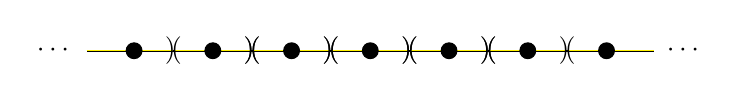
\begin{tikzpicture}
        \draw[step=1, black, thick] (-3.6, 0) -- (3.6, 0);
        \draw[yellow] (-3.6, 0) -- (-2.51, 0);
        \draw[yellow] (2.51, 0) -- (3.6, 0);
        \foreach \x in {-2, -1, 0, 1, 2} {
            \draw[yellow] (\x - 0.49, 0) -- (\x + 0.49, 0);
            \node at (\x - 0.5, 0) {$)\!($};
            \node at (\x + 0.5, 0) {$)\!($};
            \draw[fill=black] (\x, 0) circle (0.1);
        }
        \foreach \x in {-4, 4} {
            \node at (\x,0) {$\cdots$};
        }
        \draw[fill=black] (-3, 0) circle (0.1);
        \draw[fill=black] (3, 0) circle (0.1);
    \end{tikzpicture}
    \caption{The $\Z$ lattice packing in dimension $1$.}
    \label{Ch1:Fig:Z_Lattice_Packing_1D}
\end{figure}

In dimension $2$, \Cref{Ch1:Prob:SpherePacking_n}, also known as the circle packing problem, turns out to be more interesting. A reasonable strategy for finding the densest packing is to `stack' the $\Z$ lattice packing from dimension $1$ onto itself in some manner, turning these intervals into circles of the same radius. The question remains how to do this optimally.

One natural way of doing this is to stack the circles on top of themselves, turning $\Z$ into the lattice $\Z^2$, where circles are centred at points with integer coordinates: see \Cref{Ch1:Subfig:Z2_lattice_packing_2D}. Unfortunately, this packing turns out to be sub-optimal. A better candidate is the $A_2$ lattice packing: see \Cref{Ch1:Subfig:A2_lattice_packing_2D}. This packing is sometimes referred to as the \textit{honeycomb packing} due to the fact that every circle has six neighbours, whose centres form the vertices of a regular hexagon.

It is well-known that the honeycomb packing is optimal in $\R^2$. The original proof of this fact is attributed to Thue \cite{Thue}, but there are many proofs in the literature. One is outlined by Hales in \cite[p. 442]{CannonHoney}. An intuitive way of convincing oneself of Thue's theorem is that it is not possible for a circle in a given row to be in contact with more than $2$ circles in the rows above and below, meaning the $A_2$ packing cannot be improved. See \Cref{Ch1:Subfig:Kepler_Original_1}.

\begin{figure}[htb]
    \centering
    \begin{subfigure}{0.48\linewidth}
        \centering
        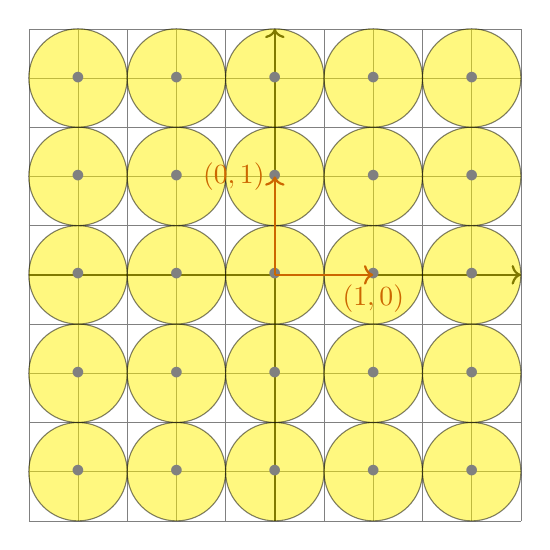
\begin{tikzpicture}[scale=1.25]
            \drawplane
            \foreach \x in {-2, -1, 0, 1, 2} {
                \foreach \y in {-2, -1, 0, 1, 2} {
                    \latticecircle{\x}{\y}
                }
            }
            \draw[->, color=brown, thick] (0,0) -- (1,0) node[anchor=north] {$\parenth{1, 0}$};
            \draw[->, color=brown, thick] (0,0) -- (0,1) node[anchor=east] {$\parenth{0, 1}$};
        \end{tikzpicture}
        \subcaption{The $\Z^2$ lattice packing.}
        \label{Ch1:Subfig:Z2_lattice_packing_2D}
    \end{subfigure}
    \begin{subfigure}{0.48\linewidth}
        \centering
        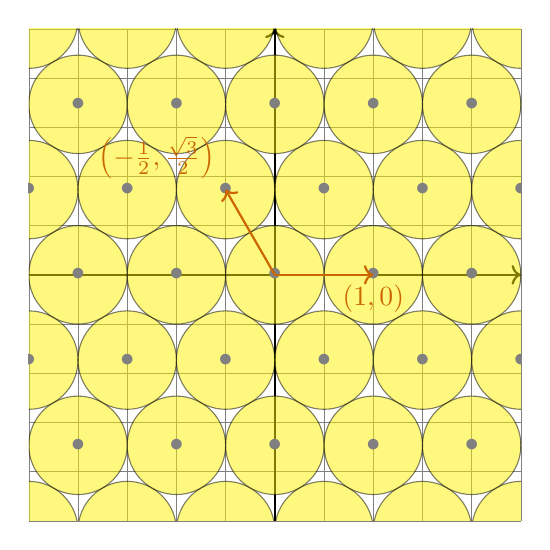
\begin{tikzpicture}[scale=1.25]
            \drawplane
            \clip (-2.5, -2.5) rectangle ++(5, 5);
            \foreach \x in {-4, -3, -2, -1, 0, 1, 2, 3, 4} {
                \foreach \y in {-3, -2, -1, 0, 1, 2, 3} {
                    \latticecircle{\x - \y * 0.5}{\y * 0.8660254038}
                }
            }
            \draw[->, color=brown, thick] (0,0) -- (1,0) node[anchor=north] {$\parenth{1, 0}$};
            \draw[->, color=brown, thick] (0,0) -- (-0.5,0.8660254038) node[anchor=south east] {$\parenth{-\frac{1}{2}, \frac{\sqrt{3}}{2}}$};
        \end{tikzpicture}
        \subcaption{The $A_2$ lattice packing.}
        \label{Ch1:Subfig:A2_lattice_packing_2D}
    \end{subfigure}
    \caption{Circle packings covering the square $\setst{\parenth{x, y} \subset \R^2}{-2.5 \leq x, y \leq 2.5}$.}
    \label{Ch1:Fig:Circle_Packings_2D}
\end{figure}

In dimension $3$, too, it is tempting to replicate this strategy: we can stack the $A_2$ packing on top of itself, in layers instead of rows, attempting to maximise the number of neighbours of a sphere. From trial and error, we see that a sphere cannot be in contact with more than three neighbours from the layer below. This suggests that the optimal sphere packing in dimension $3$ is given by stacking honeycomb arrangements on top of each other with spheres in each layer being nestled in the gaps between three spheres in the layer below.

\begin{wrapfigure}[28]{r}{0.27\linewidth}
    \centering
    \begin{subfigure}{\linewidth}
        \centering
        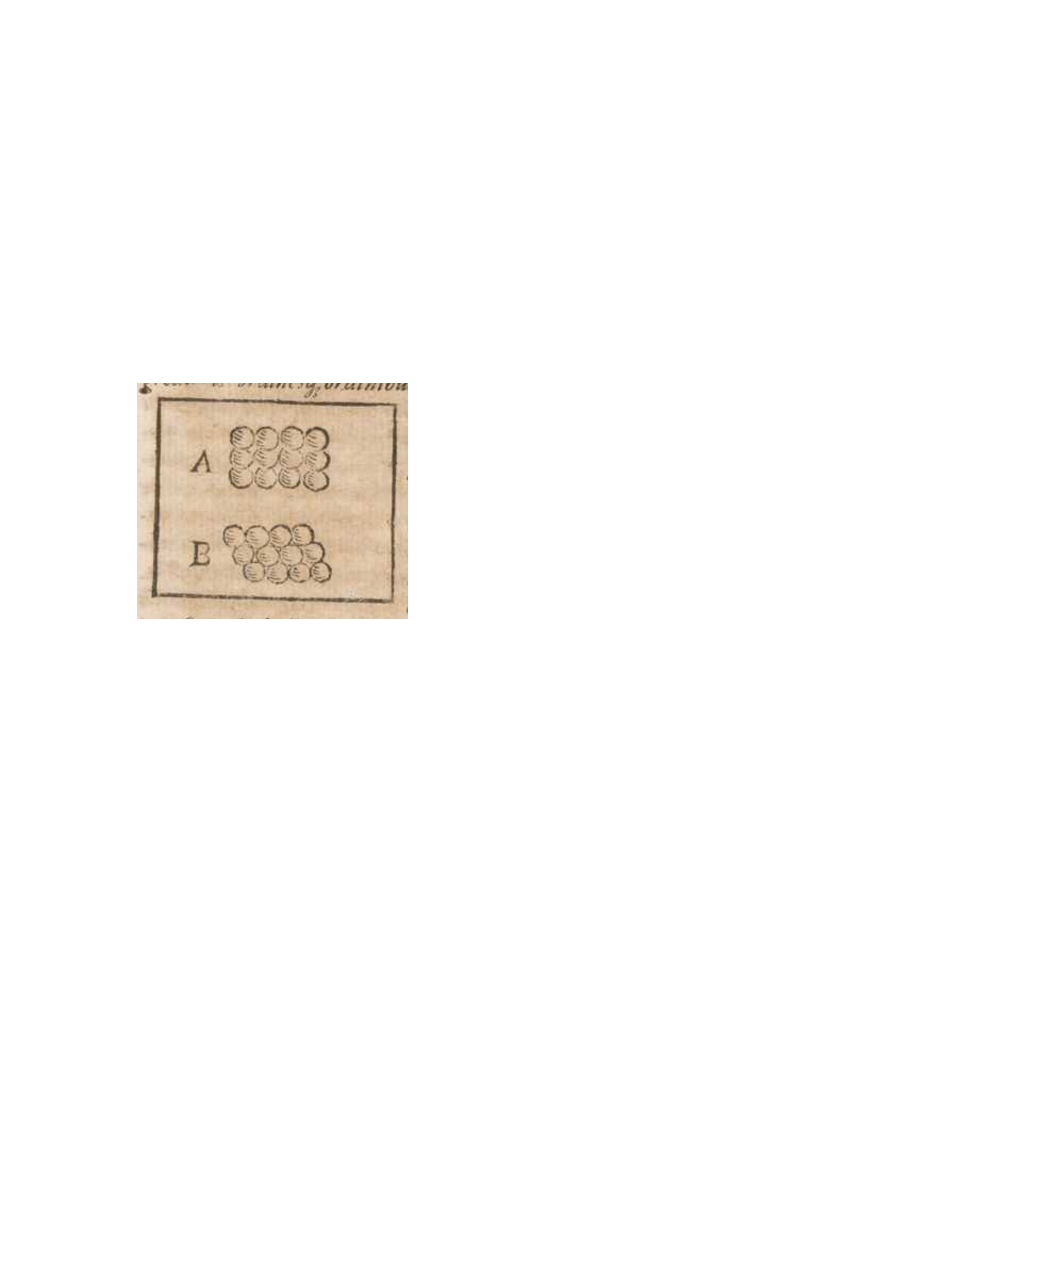
\includegraphics[width=\linewidth]{Chapters/1_Intro/Images/Kepler_1.pdf}
        \caption{}
        \label{Ch1:Subfig:Kepler_Original_1}
    \end{subfigure}
    \begin{subfigure}{\linewidth}
        \centering
        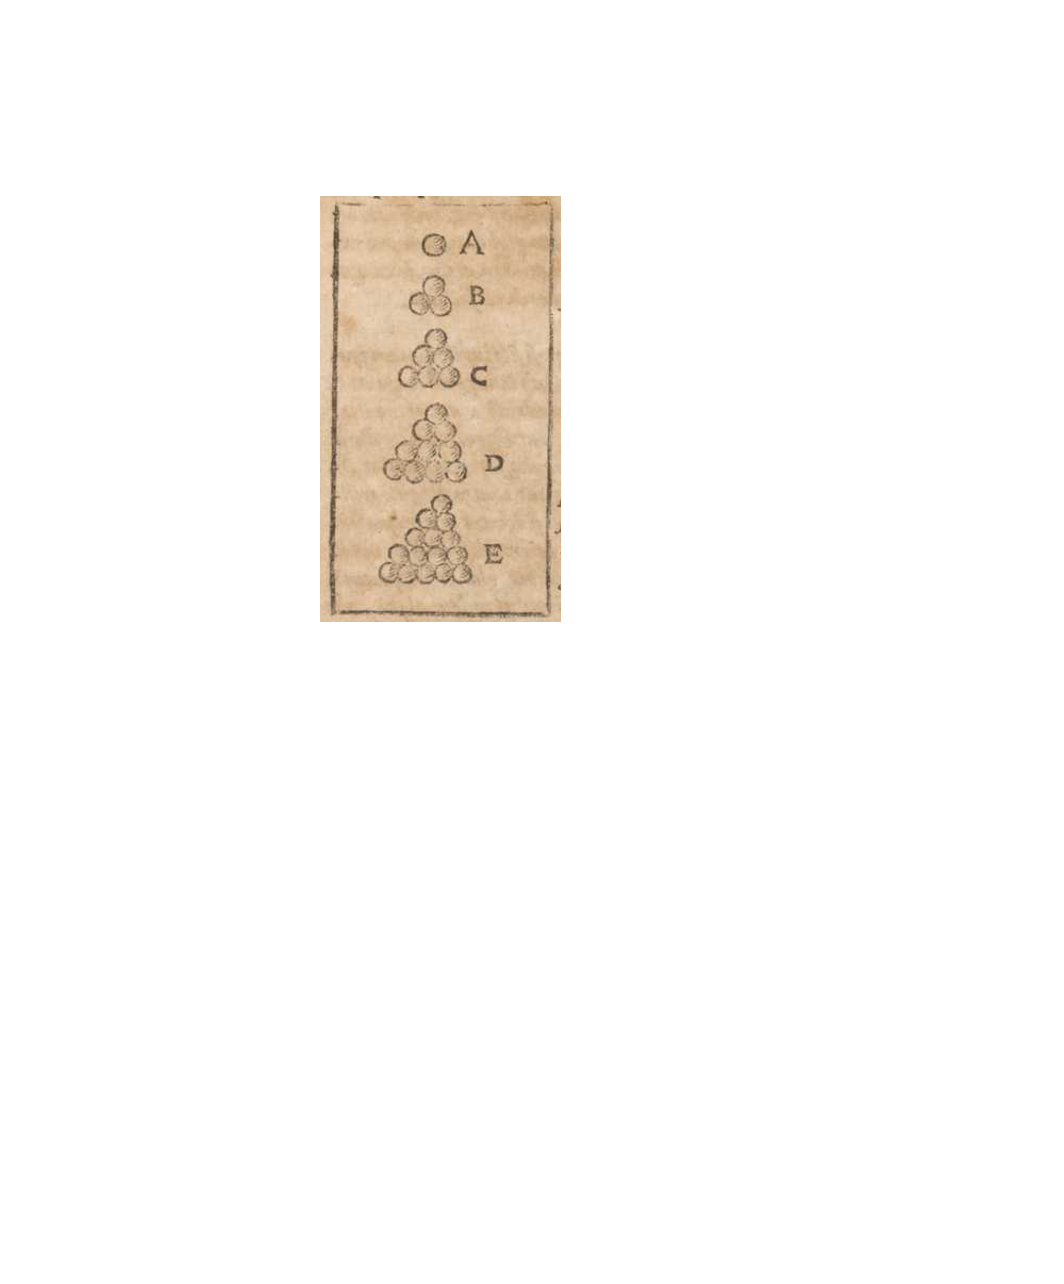
\includegraphics[width=\linewidth]{Chapters/1_Intro/Images/Kepler_2.pdf}
        \caption{}
        \label{Ch1:Subfig:Kepler_Original_2}
    \end{subfigure}
    \caption{Diagrams from an essay written by Johannes Kepler in Latin in 1611 \cite{KeplerSnowflake}.}
\end{wrapfigure}

As it turns out, unlike dimension $2$, this characterisation not describe a unique packing: spheres are simply too large! See \Cref{Ch1:Fig:2_Optimal_3D_Packings}. One can construct infinitely many locally similar, globally different sphere packings in $\R^3$, all of which are as dense as possible, by varying how successive layers are placed.

\begin{figure}[bt]
    \centering
    \begin{subfigure}{0.48\linewidth}
        \centering
        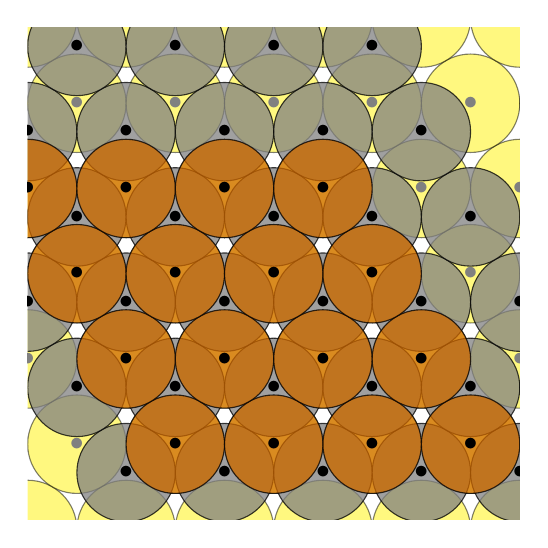
\begin{tikzpicture}[scale=1.25]
            \clip (-2.5, -2.5) rectangle ++(5, 5);
            \foreach \x in {-4, -3, -2, -1, 0, 1, 2, 3, 4} {
                \foreach \y in {-3, -2, -1, 0, 1, 2, 3} {
                    \latticecircle{\x - \y * 0.5}{\y * 0.8660254038}
                }
            }
            \foreach \x in {-3, -2, -1, 0, 1, 2} {
                \foreach \y in {-3, -2, -1, 0, 1, 2} {
                    \latticecirclegrey{\x - \y * 0.5}{\y * 0.8660254038 + 0.5773502692}
                }
            }
            \foreach \x in {-2, -1, 0, 1} {
                \foreach \y in {-2, -1, 0, 1} {
                    \latticecirclebrown{\x - \y * 0.5}{\y * 0.8660254038}
                }
            }
        \end{tikzpicture}
        \subcaption{}
        \label{Ch1:Subfig:3D_Triangular_Stacking}
    \end{subfigure}
    \begin{subfigure}{0.48\linewidth}
        \centering
        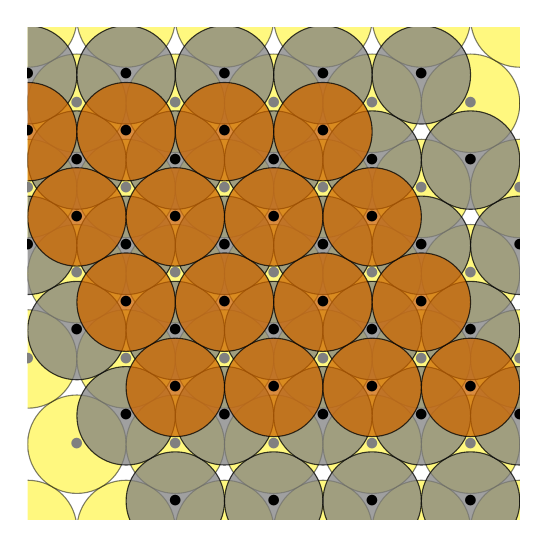
\begin{tikzpicture}[scale=1.25]
            \clip (-2.5, -2.5) rectangle ++(5, 5);
            \foreach \x in {-4, -3, -2, -1, 0, 1, 2, 3, 4} {
                \foreach \y in {-3, -2, -1, 0, 1, 2, 3} {
                    \latticecircle{\x - \y * 0.5}{\y * 0.8660254038}
                }
            }
            \foreach \x in {-2, -1, 0, 1, 2, 3} {
                \foreach \y in {-2, -1, 0, 1, 2, 3} {
                    \latticecirclegrey{\x - \y * 0.5}{\y * 0.8660254038 - 0.5773502692}
                }
            }
            \foreach \x in {-2, -1, 0, 1} {
                \foreach \y in {-2, -1, 0, 1} {
                    \latticecirclebrown{\x - \y * 0.5}{\y * 0.8660254038 + 0.5773502692}
                }
            }
        \end{tikzpicture}
        \subcaption{}
        \label{Ch1:Subfig:3D_Hexagonal_Stacking}
    \end{subfigure}
    \caption{Two different ways of stacking the honeycomb packing on itself.}
    \label{Ch1:Fig:2_Optimal_3D_Packings}
\end{figure}

This observation is not novel. In a 1611 essay whose title has been translated from Latin as \textit{The Six-Cornered Snowflake} \cite{KeplerSnowflake}, Johannes Kepler asserted that spheres cannot be more tightly packed together than they are in a tetrahedral arrangement: see \Cref{Ch1:Subfig:Kepler_Original_2}. This result became known as the Kepler Conjecture, and it went unproven for over three centuries, until 2005 that a paper proving it, written by Thomas Hales, was published \cite{HalesKeplerInformal}.

The complexity of the sphere packing problem in dimension $3$ is illustrated not only by the time elapsed between Kepler's original assertion and a proof being published but also by the length of Hales's paper. Indeed, in an expository account of his proof published in 2000, five years before the publication of the full paper in the Annals, Hales recounted how a jury of twelve referees, despite having been in deliberation for over a year, had yet to make a ``thorough, independent check of the computer code'' he had written to perform the elaborate calculations on which ``every aspect of [his proof] is based'' \cite{CannonHoney}. In January 2003, at the Joint Math Meetings in Baltimore, USA, Hales announced that he intended to formally verify his proof \cite{HalesKeplerFormal}, in what he termed the Flyspeck project. The paper authored by Hales and his collaborators on their successful formalisation of his argument was only published in 2017. Therefore, not only did the Kepler Conjecture take close to 400 years to solve, but it took nearly two decades to eliminate any doubt as to the correctness of the solution. This project aims to formalise a result of a similar flavour in a significantly shorter timeframe.
\section{The Work of Maryna Viazovska}
\section{The Formalisation Movement}
\section{Progress in Formalising Viazovska's Solution in Dimension $8$}

% Do I want to turn this into a separate chapter and toss in section 1.5?
\section{The Scope of this Project}
\chapter{A Roadmap to Constructing the Magic Function}
\thispagestyle{empty}

We mentioned, in the introduction, that the scope of this project is to construct Viazovska's Magic Function in Lean and prove that it satisfies certain specific properties, such as satisfying the hypotheses of the \CELP. In this chapter, we will outline the steps we will take to achieve this goal. In particular, we will list all the conditions we need to prove that the Magic Function satisfies. Our approach will be to construct the Magic Function in terms of two intermediary functions. Proving it satisfies the necessary conditions will then be a matter of proving that these intermediary functions satisfy certain properties. We will list these properties as well.

\section{On Schwartz Functions}
\section{The \CEC}
\section{The Desired Properties of the Magic Function}

% Beyond Schwartz and the \CEC, explain why it needs to be radial and have double zeroes at lattice points. Fourier Eigenfunction bit would be nice as well.
\section{The Magician's Assistants: $a$ and $b$}

% \appendix
% \chapter{First Appendix}

%%%%%%%%%%%%%%%%%%%%%%%%%%%%%%%%%%%%%
\bibliography{References/bibliography.bib}
\thispagestyle{empty}
%%%%%%%%%%%%%%%%%%%%%%%%%%%%%%%%%%%%%

\end{document}